\documentclass[letter,11pt]{article} % Tamaño de página y letra, tipo de documento
\usepackage[top = 2.0cm, bottom = 2.0cm, left = 2.0cm, right = 2.0cm]{geometry}

%% Comandos para codificación de archivo
\usepackage[utf8]{inputenc}
\usepackage[spanish,es-tabla]{babel}
\spanishdecimal{.}

%%%%%%%%%%%%%%%%%%%%%%%%%%%%%%%%%%%%%%%%%%%%%%%%
%% Bibliotecas útiles %%
\usepackage{multirow} % Múltiples renglones
\usepackage{multicol} % Múltiples columnas
\usepackage{booktabs} % Tablas más estéticas
\usepackage{graphicx} % Agregar figuras
\usepackage{setspace}  % Quita sangría de inicio de párrafos
\setlength{\parindent}{0in}
\usepackage{float} % Control de ubicación de figuras
\usepackage{fancyhdr} % Formato de encabezados
\usepackage{amsmath,mathtools,amsfonts,amssymb} % Símbolos matemáticos
\usepackage{xcolor} % Texto y ecuaciones en color
\usepackage{pdfpages} % Insertar PDFs
\usepackage{hyperref}
\newcommand{\Heaviside}{\mathrm{H}}
%%%%%%%%%%%%%%%%%%%%%%%%%%%%%%%%%%%%%%%%%%%%%%%%
%% Encabezado y pie de página %%
\pagestyle{fancy}  
\fancyhf{} 
%%%%%%%%%%%%%%%%%%%%%%%%%%%%%%%%%%%%%%%%%%%%%%%%
\lhead{\footnotesize Simulación Rover Tarea 02} 
\rhead{\footnotesize LIRA} 
\cfoot{\footnotesize \thepage} 
%%%%%%%%%%%%%%%%%%%%%%%%%%%%%%%%%%%%%%%%%%%%%%%%
%% Aquí comienza la edición del documento
\usepackage{float}
\begin{document}
	\thispagestyle{empty} % Sin encabezado en la primera página
	
	%%%%%%%%%%%%%%%%%%%%%%%%%%%%%%%%%%%%%%%%%%%%%%%%
	%% Datos para la primera página
	\begin{tabular} {p{15cm} p{2cm}}
		&  \multirow{5}{*}{\includegraphics[scale=0.11]{UNAM_INGENIERIA}}\\
		{\large \bf Laboratorio de Innovación y Robótica Avanzada} & \\
		{\large \bf LIRA} & \\
		UNAM | FI & \\
		&  \\
		\hline
	\end{tabular} 
	
	\vspace*{0.3cm} 
	
	\begin{center}
		{\bf {\normalsize Primer acercamiento a Webots}} \\
	\end{center}
	\vspace{2mm} 
	%Documento
	
	\textbf{¿Qué es Webots?} \\
	
	Webots es una potente plataforma profesional de simulación robótica, gratuita y de código abierto, utilizada tanto en la industria como en la investigación. Te permite crear entornos 3D detallados y replicar propiedades físicas complejas como masa, inercia y fricción para una gran variedad de robots, ya sean con ruedas, piernas o aéreos.	Lo que lo hace especialmente poderoso es su capacidad para programar el comportamiento de los robots usando lenguajes populares como Python, C++ o MATLAB. Cuenta con una extensa biblioteca de sensores (cámaras, LiDAR, GPS), actuadores y modelos de robots comerciales listos para usar. Uno de sus mayores beneficios es la facilidad para transferir el código probado en la simulación a un robot físico real, lo que lo convierte en una herramienta ideal para la educación, la investigación y la participación en competiciones internacionales como la RoboCup.
	
	\vspace{2mm}
	
	\textbf{¿Qué compone una simulación de Webots?}
	
	Esta compuesta por cuatro elementos: el entorno de simulación, modelos robóticos, el controlador y el motor de físicas
		\begin{itemize}
			\item \textbf{Entorno de Simulación:} Define el escenario físico: suelos, paredes, obstáculos; condiciones ambientales, posición incial de los robots, entre otras cosas. Esto puede ser editado mediante el "Scene Tree", el cual lista todos los objetos.
			El escenario es un archivo de texto con la extensión .wbt
			\item \textbf{Modelos Róboticos:} Son los individuos del mundo creado, más allá de ser un modelo 3D, son un conjunto de nodos que definen las capacidades propias del robot. Se encuentra compuesto por las siguientes partes:
			\begin{itemize}
				\item \textbf{Cuerpo:} son las partes físicas del robot.
				\item \textbf{Actuadores:} son los componentes que le permiten moverse e interactuar.
				\item \textbf{Sensores:} Son los componentes que le permiten al robot percibir su entorno.
			\end{itemize}
			\item \textbf{Motor de Físicas:} Es la parque se asegura de que el mundo actúe según las leyes de la física. Webots utiliza una versión modificada del Open Dynamics Engine. Se conforma de: 
			\begin{itemize}
				\item \textbf{Responsabilidades:} Se encarga de la simulación siga las fisicas.
				\item \textbf{Detección de Colisiones:} Identifica cuándo dos objetos se tocan.
				\item \textbf{Dinámica de Cuerpos Rígidos:} Calcula cómo las fuerzas y los torques afectan el movimiento y rotación de los objetos.
				\item \textbf{Fricción:} Simula la fricción estática y cinética entre las superficies.
			\end{itemize}
			 
		\end{itemize}
		
		Una vez desmenusado y explicado como funciona y que compone el software, se puede empzar a interactuar con el sistema de simulaciones Webots.
		Para más información se puede visitar la página oficial de Webots: https://cyberbotics.com/doc/guide/introduction-to-webots
		
		\clearpage 
		\textbf{Interfaz de Webots} \\[0.3cm] % un poco de espacio
		
		\begin{figure}[h!]
			\centering
			\includegraphics[width=0.6\linewidth]{ImagenesTarea/Interfaz}
			\caption{Interfaz}
			\label{fig:interfaz}
		\end{figure}
		
		La interfaz gráfica esta compuesta de: 
		\begin{itemize}
			\item \textbf{3D window}: muestra lo que sucede en la simulación.
			\item \textbf{Scene Tree}: representación jerarquica de la simulación.
			\item \textbf{Text Editor}: permite editar el código fuente.
			\item \textbf{Console}: Muestra la compilación y el controlador
		\end{itemize}
		En la barra del menú tenemos: \textbf{File, Edit, View, Simulation, Build, Overlays, Tools y Help}
		\vspace{2mm}
		
		Para tener una mejor comprensión del entorno de Webots, comencemos abriendo un ejemplo de los que vienen predeterminados por el programa.
		
		En nuestra terminal ejecutaremos la siguiente linea de comando: 
		\begin{center}
			\textbf{cd /usr/local/webots/projects/samples/tutorials/worlds/}
		\end{center}
		Esto desplegará los ejemplos disponibles del programa. En nuestra terminal ejecutaremos: \texttt{webots my\_first\_simulation.wbt}
		
		
		Después se abrira la siguiente ventana y veremos la siguiente simulación. \\[2mm]
		
		\begin{figure}[H] % <--- ¡Este es el cambio principal!
			\centering
			\includegraphics[width=0.6\linewidth]{ImagenesTarea/ejemplo}
			\caption{Ejemplo}
			\label{fig:ejemplo}
		\end{figure}
		
		
		La simulación desplegada mostrará un E-puck que solo avanzará en línea recta hasta chocar con la pared.
		
		Si hacemos click ziquierdo sobre el robot, se pueden observar las líneas que delimitan su forma, vendrían siendo su contorno geométrico así como los tres ejes (x, y, z) y sus respecticas rotaciones (roll, pitch, yaw).
		
		\begin{figure}[H]
			\centering
			\includegraphics[width=0.6\linewidth]{"../Pictures/Screenshots/Screenshot from 2025-10-01 23-53-39"}
			\caption{Contorno Geométrico}
			\label{fig:screenshot-from-2025-10-01-23-53-39}
		\end{figure}
		
		Si seleccionamos alguna de estas, se puede modificar la posición o alguno del objeto (solo si esta pausada la simulación) se mostrara una leyenda que indicará su posición o ángulo con respecto a sus offsets. 
		
		También pueden usarse:
		\begin{itemize}
			\item \textbf{Shift + flecha hacia arriba} y click derecho para mover el objeto
			\item \textbf{Shift + flecha hacia arriba} y click izquierdo para rotar el objeto
		\end{itemize}
		
		Otras interacciones que pueden tenerse con la 3D window, son la aplicación de efectos físicos: como el \textbf{torque y fuerza}
		\begin{itemize}
			\item \textbf{Torque}: \textbf{Ctrl + Alt } y click derecho, se observará un vector amarillo el cuál mostrara un marcador del torque aplicado al obejto.
			\item \textbf{Fuerza}: \textbf{Ctrl + Alt } y click izquierdo, se observará un vector naranja el cuál mostrara un marcador de la fuerza aplicada al obejto.
		\end{itemize}
		Ambas varían su magnitud en función de la longitud del vector.
	
		Hacer click derecho sobre el objeto despliega una ventana que muestra diferentes acciones disponibles para el mismo. Se recomienda probar cada una para familiarizarse con las acciones que hacen, si algo desaparece o cambia, solo refresca la simulación sin guardar. 
		Las últimas 6 opciones, permiten acceder al código que compone el comportamiento del robot así como del mundo construido. 
		
		
		\begin{figure}[H]
			\centering
			\includegraphics[width=0.5\linewidth]{"../Pictures/Screenshots/Screenshot from 2025-10-02 00-15-06"}
			\caption{Ventana de acciones}
			\label{fig:screenshot-from-2025-10-02-00-15-06}
		\end{figure}
		
		Para poder observar la camara u otros sensores disponibles, seleccione la opción de \textbf{Overlays} y se mostrarán los que están disponibles para el robot en uso. 
		Para el E-puck, seleeccione \textbf{Show 'camera' overlay} y se desplegará una ventana negra en la parte superior de la simulación. Para poder inciarla seleccione la opción \textbf{Show Robot window} desplegandose una ventana como esta.
		\begin{figure}[h]
			\centering
			\includegraphics[width=0.4\linewidth]{ImagenesTarea/screenshot001}
			\caption{Robot window}
			\label{fig:screenshot001}
		\end{figure}
		
		Seleccione el boton de \textbf{Enable All}, seleecione \textbf{Refresh} en Simultaion y Upload HEX..
		¿Qué cambios hubo en la simulación? \\[2mm]
		
		En nuestra terminal ejecutaremos: \textbf{Crtl+ C} y escribiremos \texttt{webots 4\_wheels\_robot.wbt 
		} 
		
		La silumación desplegada es de un carro que evita chocar con las paredes. \\[2mm]
		
		Del lado derecho se encuentran la sección \textbf{Scene Tree y Editor Field}
		\begin{figure}[H]
			\centering
			\includegraphics[width=0.2\linewidth]{ImagenesTarea/screenshot002}
			\caption{Barra lateral}
			\label{fig:screenshot002}
		\end{figure}
		
		El \textbf{Scene Tree} es una lista organizada que muestra  todos los elementos que existen en la simulación (robots, luces, obstáculos, suelo, etc.) y como estos se relacionan entre si.
		\begin{itemize}
			\item \textbf{Estructura Jerárquica:} Los objetos se encuentran anidados unos dentro de otros.
			\item \textbf{Organización y Navegación:} Permite encontrar y seleccionar rápidamente cualquier objeto en la escena, sin importar si es visible o no en la ventana 3D
			\item \textbf{Contenedor Global:} Ese nodo es especial, ya que maneja las reglas globales queafectan a todo el mundo, como la gravedad o la configuración de la dísica.
		\end{itemize}
		
		Al seleccionar uno de los objetos que hay en el \textbf{Scene Tree}, se activa el \textbf{Field Editor} y funcioa como la hoja de propiedades o el panel de control de ese objeto específico.
		\begin{itemize}
			\item \textbf{Visualización de Atributos:} Muestra todas las características y parámetros dek ibjeto seleccionado.
			\item \textbf{Modificación de Propiedades:} Permite cambiar los valores de estos campos. Se puede ajustar números, seleccionar opciones de menús desplegables o escribir texto para configurar el comportamiento y la apariencia del objeto.
		\end{itemize}	
		
		 Seleccione el nodo Robot, se desplegará todos los nodos relacionados con el robot. Seleccione \textbf{children} y luego \textbf{DEF BODY Shape} mostrando los nodos ligados a la parte física del robot. 
		 Seleccione \textbf{geometry Box} y \textbf{size} esto activará el \textbf{Editor Field} a continuación modifique el aspecto físico del robot. Para deshacer los cambios solo reinice la simulación. \\[2mm]
		 
		 Así como se puede interactuar con el aspecto, también se puede modificar el comportamiento de los sensores y actuadores del robot.
		 
		 Dentro de \textbf{DEF DS\_RIGHT DistanceSensor} busqué \textbf{lookupTable} y coloque los valores a 0 y \textbf{DEF DS\_LEFT DistanceSensor} eliminelo.
		 \textbf{lookupTable }traduce la distancia que mide el sensor a un valor numérico que entiende el robot. Por ejemplo: "si mido 0.1 metros, devuelve el valor 1000". entonces al colocarlos en 0 el sensor no sabrá qué valor devolver, por lo que siempre enviará un 0. Para el controlador del robot, un 0 significa "no hay obstáculo", por lo que el sensor queda efectivamente desactivado.
		 
		 Eliminar \textbf{DEF DS\_LEFT DistanceSensor} quita por completo el sensor izquierdo. Lo que genera que el robot se quedé dando vueltas ya que entra en un bucle de rotación.
		 \\[2mm]
		 Reinicie la simulación y modifique \textbf{lookupTable }para que la distancia de detección aumente y en otra disminuya. \\[2mm]
		 
		 \clearpage
		 \textbf{ROVER}
		 
		 Un \textit{rover} o astromóvil es un vehículo de exploración diseñado para desplazarse sobre la superficie de un planeta u objeto astronómico. Estos dispositivos son empleados en misiones espaciales para recopilar datos e imágenes, así como para realizar análisis de muestras de suelo, rocas y atmósfera. Su uso resulta fundamental para la exploración remota de cuerpos celestes como la Luna, Marte y otros planetas o asteroides de interés científico. 
		 \\[2mm]
		 Los objetivos y características de un astromóvil pueden variar según la misión o el entorno en el que operará. Entre los principales se encuentran:
		 \begin{itemize}
		 	\item Investigación científica
		 	\item Búsqueda de signos de vida
		 	\item Análisis geológico
		 	\item Búsqueda y aprovechamiento de recursos
		 \end{itemize} 	
		 Además, los rovers suelen incorporar sistemas avanzados que les permiten operar de forma autónoma o semiautónoma. Entre sus principales subsistemas destacan: la movilidad, el sistema de energía (paneles solares o baterías), las comunicaciones, los instrumentos científicos y los sistemas de navegación y control.
		 
		 \\[2mm]
		 Al igual que los vehículos terrestres, los rovers pueden clasificarse en distintos tipos según su aplicación y el entorno donde trabajen:
		 \begin{itemize}
		 	\item Rovers planetarios
		 	\item Rovers lunares
		 	\item Rovers para asteroides
		 	\item Rovers de exploración submarina o terrestre
		 \end{itemize}
		 
		 \begin{figure}[H]
		 	\centering
		 	\begin{minipage}{0.45\linewidth}
		 		\centering
		 		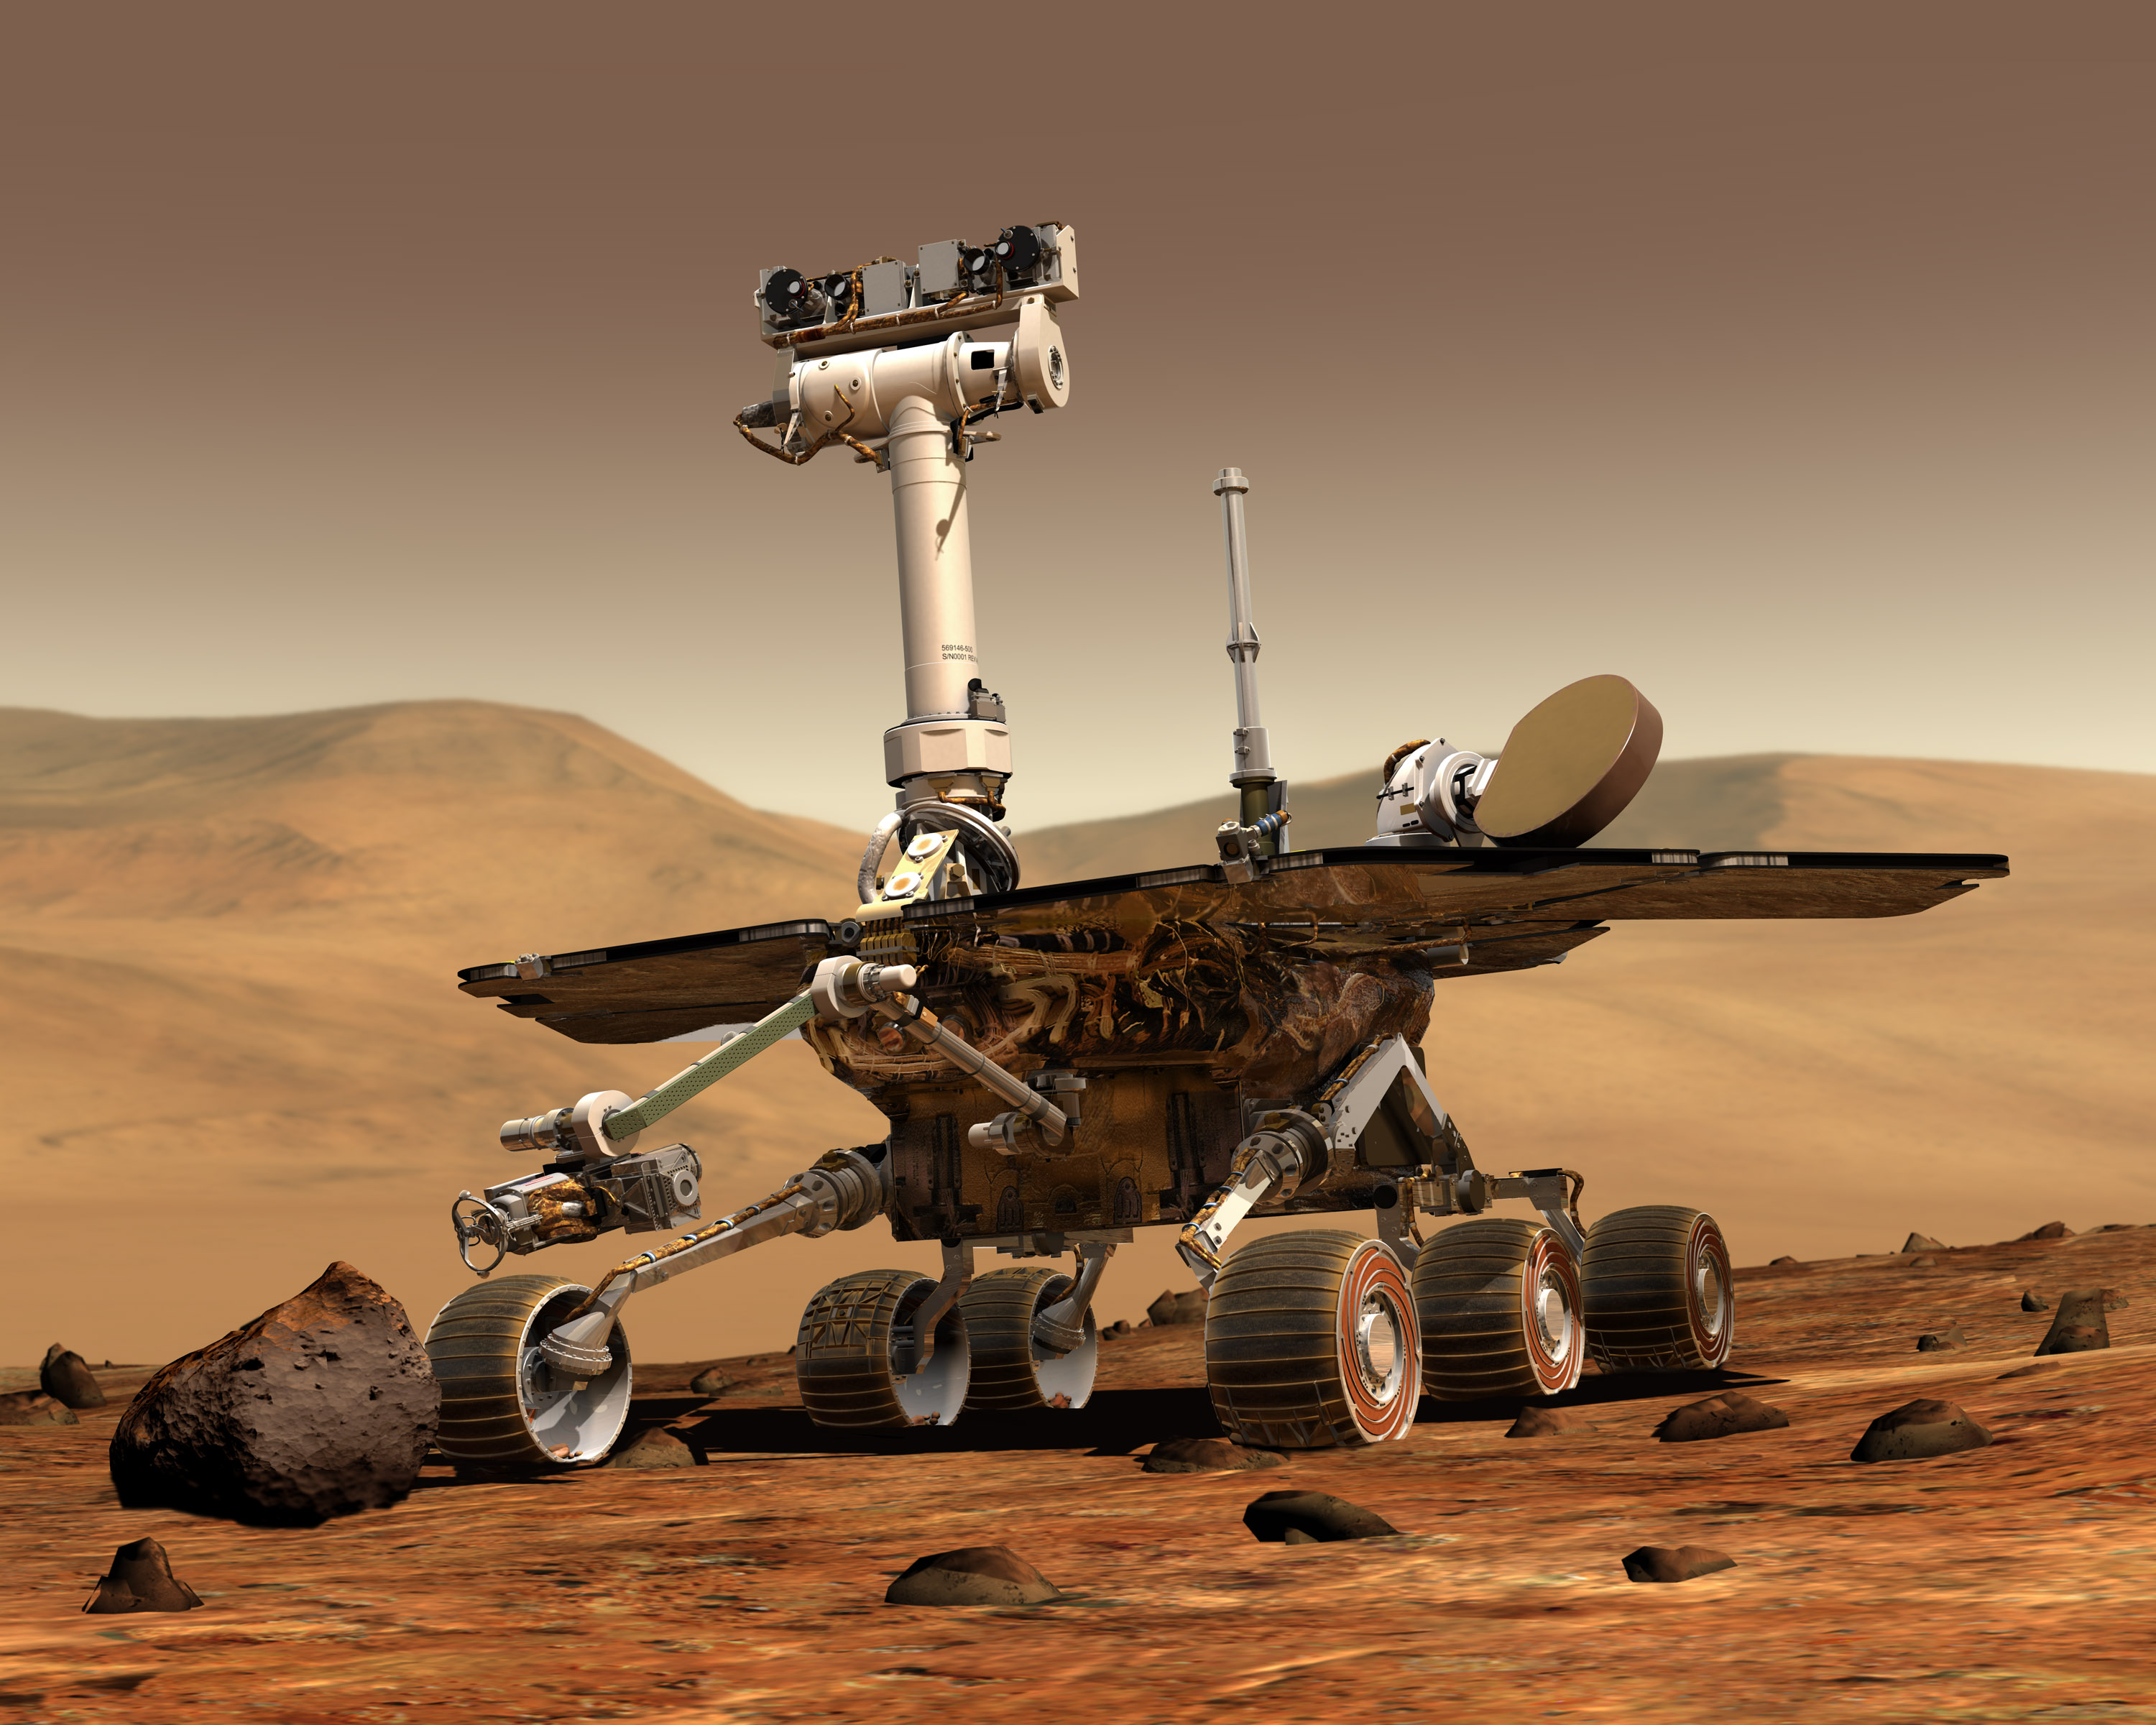
\includegraphics[width=\linewidth]{ImagenesTarea/screenshot003}
		 		\caption{Rover de exploración marciana.}
		 		\label{fig:screenshot003}
		 	\end{minipage}
		 	\hfill
		 	\begin{minipage}{0.45\linewidth}
		 		\centering
		 		\includegraphics[width=\linewidth]{ImagenesTarea/screenshot005}
		 		\caption{Prototipos de rover para pruebas terrestres.}
		 		\label{fig:screenshot005}
		 	\end{minipage}
		 \end{figure}
		 
		 Para las simulaciones y posteriormente las prácticas físicas, se empleará un modelo de rover simplificado que permite comprender los principios de locomoción, control y navegación autónoma. Este tipo de modelos facilita el diseño e implementación de algoritmos de control mediante software como \textbf{Webots} o entornos de desarrollo con \textbf{ROS 2}, donde es posible recrear sensores virtuales, cámaras, motores y terrenos de prueba realistas.
		 
		 \\[2mm]
		 En la siguiente figura se muestra el modelo utilizado para la simulación, el cual sirve como base para experimentar con comandos de movimiento, adquisición de datos y validación de estrategias de control antes de su implementación en un sistema físico.
		 
		 \begin{figure}[H]
		 	\centering
		 	\includegraphics[width=0.5\linewidth]{ImagenesTarea/screenshot006}
		 	\caption{Modelo de rover empleado para simulación en Webots.}
		 	\label{fig:screenshot006}
		 \end{figure}
		 
		 Para probar esta simulación haremos lo siguiente:
		 \begin{center}
		 	\textbf{cd PAPIME\_PE103825/ros2\_ws/}
		 	
		 	\textbf{colcon buildsource} 
		 	
		 	\textbf{install/setup.bash}
		 	
		 	\textbf{ros2 launch rover\_control rover\_launch.py}
		 \end{center}	
		 
		
		La simulación consiste en el rover mostrado anteriormente, desplazandose en línea recta a una velocidad de 5 m/s.
		
		\\[2mm]
		Para modificar la velocidad, así como el angulo de desplazamiento, ejecute el sigueinte comando en la terminal. 
		\begin{center}
			\textbf{cd src/hardware/rover\_control/rover\_control/} 
		\end{center}
		Y ejecute el script de python: \textbf{rover\_control.py}. En el modificará las sigueintes líneas.
		\begin{figure}[H]
			\centering
			\includegraphics[width=0.4\linewidth]{ImagenesTarea/screenshot008}
			\caption{Parámetros}
			\label{fig:screenshot00}
		\end{figure}
		
		\\[2mm]
		El parámetro \textbf{linear.x} controla la velocidad angular (en radianes por segundo)  
		, mientras que \textbf{angular.z} controla la velocidad lineal 
		(en metros por segundo). 
		
		Por ejemplo:
		\begin{itemize}
			\item \texttt{linear.x = 0.0}, \texttt{angular.z = 0.5} → movimiento recto hacia adelante.
			\item \texttt{linear.x = 1.0}, \texttt{angular.z = 0.0} → giro sobre su propio eje hacia la izquierda.
			\item \texttt{linear.x = -1.0}, \texttt{angular.z = 0.0} → giro sobre su propio eje hacia la derecha.
			\item \texttt{linear.x = 0.5}, \texttt{angular.z = 0.5} → avance con giro leve a la izquierda.
			\item \texttt{linear.x = -0.1}, \texttt{angular.z = 0.5} → avance con giro leve a la derecha.
		\end{itemize}
		
		
		\\[2mm]
		Si únicamente modifica los valores dentro del script \texttt{rover\_control.py}, 
		basta con guardar los cambios y volver a lanzar la simulación en Webots.  
		Sin embargo, si modifica la estructura del paquete (por ejemplo, el archivo \texttt{setup.py}, 
		\texttt{launch} o el \texttt{URDF}), deberá ejecutar nuevamente:
		\begin{center}
			\textbf{colcon build} \\
			\textbf{source install/setup.bash}
		\end{center}
		para aplicar los cambios correctamente.
		\\[3mm]	
		
		
		\textbf{Conclusión} \\[2mm]
		El uso de Webots en conjunto con ROS 2 permite integrar la simulación de robots móviles dentro de un entorno físico virtual controlado mediante nodos y tópicos, reproduciendo de manera precisa el comportamiento real de sistemas robóticos. A través de esta práctica se comprendió cómo un plugin de Webots puede conectarse con ROS 2 para recibir comandos de movimiento mediante mensajes del tipo \textbf{geometry\_msgs/Twist}.\\
		
		El mensaje Twist representa las velocidades lineales y angulares de un robot, sirviendo como interfaz estándar entre los algoritmos de control y los actuadores simulados o reales. De esta forma, modificar los valores de linear.x o angular.z permite definir trayectorias, giros o desplazamientos en línea recta, replicando el mismo principio que se usa en robots físicos.
		
		Esta integración demuestra la potencia de ROS 2  para el desarrollo modular y escalable de robots, y de Webots como entorno de validación antes de llevar los sistemas al hardware real. En conjunto, ambas herramientas permiten diseñar, probar y optimizar algoritmos de navegación, control de velocidad y planificación de movimiento de manera segura y eficiente.

	
	
	
\end{document}
